% =====================================================================
%  chunks/ch04a.tex —— 原书 p.142–152（PDF 149–159）
%  第 4 章 光滑流形；§1 基本概念、光滑纤维丛、联络、示性类（上）
% =====================================================================
% [原文 p.142]
\chapter{光滑流形}

\section{基本概念。光滑纤维丛。联络。示性类}

\takeaway{本节从坐标卡与单位分解出发建立光滑流形的基本语言：切空间、张量场、微分形式与外微分；继而引入 Lie 群、光滑纤维丛与向量丛、Stiefel 与 Grassmann 流形及其分类空间；最后用联络与曲率把几何数据写成 Lie 代数值形式。}

光滑（可微）流形的拓扑与几何，是拓扑学中最重要的研究领域：整套拓扑学方法由此发源，并在此找到最富成果的应用；它与分析、尤其与当代数学物理紧密相连。光滑流形的初等理论由 Whitney 于 1930 年代中期创立。

可微流形的内蕴定义如下。它首先是一个（$n$ 维）\emph{拓扑流形}（见第 2 章 §1 末尾），即 Hausdorff 拓扑空间 $X$，存在一簇覆盖 $X$ 的开集 $V_\alpha$（$\bigcup_\alpha V_\alpha=X$），其中每个都同胚于 $\R^n$ 的某个开区域。这样的同胚
\[
\phi_\alpha:V_\alpha\to\R^n
\]
于是在每个开集（或\emph{坐标卡}（chart）、\emph{局部坐标邻域}）$V_\alpha$ 上确定\emph{局部坐标} $(x_\alpha^1,\ldots,x_\alpha^n)$。若在每个交集区域 $V_\alpha\cap V_\beta$ 上，用一组坐标表示另一组坐标的\emph{衔接函数}都是 $C^k$ 类光滑的，即欧氏 $n$ 空间相应区域之间的映射 $\phi_\alpha\phi_\beta^{-1}$、$\phi_\beta\phi_\alpha^{-1}$ 都是 $C^k$ 类函数（$k>0$），则称流形 $X$ 是 \emph{$C^k$ 类光滑的}。（若 $k=\infty$，则称流形\emph{无穷可微}，或简称\emph{光滑}。若衔接函数都是实解析的，则称\emph{实解析流形}。）

流形将记作 $M^n$、$N^k$ 等。注意衔接函数 $x_\alpha(x_\beta)$ 的 Jacobi 行列式
\[
\det(\partial x_\alpha^i/\partial x_\beta^j)
\]
在 $V_\alpha\cap V_\beta$ 上处处非零：若它在某点为零，则逆函数 $x_\beta(x_\alpha)$ 便不光滑。

在初等水平上发展研究光滑流形的技巧，需要\emph{单位分解}的存在性，即：对流形 $M^n$ 的每个开覆盖 $\{V_\alpha\}$，存在开集 $W_\alpha\subset W'_\alpha\subset V_\alpha$ 使 $\bigcup_\alpha W_\alpha=M^n$，以及定义在 $M^n$ 上的 $C^\infty$ 类实值函数 $\psi_\alpha\ge0$，满足下列性质（见图 4.1）：
\[
\psi_\alpha\equiv1\ \text{在}\ W_\alpha\ \text{上};\qquad \psi_\alpha\equiv0\ \text{在}\ W'_\alpha\ \text{之外};
\]
\[
\infty>\sum_\alpha\psi_\alpha(x)>0\ \text{对每个}\ x\in M^n;\qquad \sum_\alpha\phi_\alpha=1,\quad \text{其中}\ \phi_\alpha=\psi_\alpha/\sum\psi_\alpha.
\]

% [原文 p.143]
\begin{center}
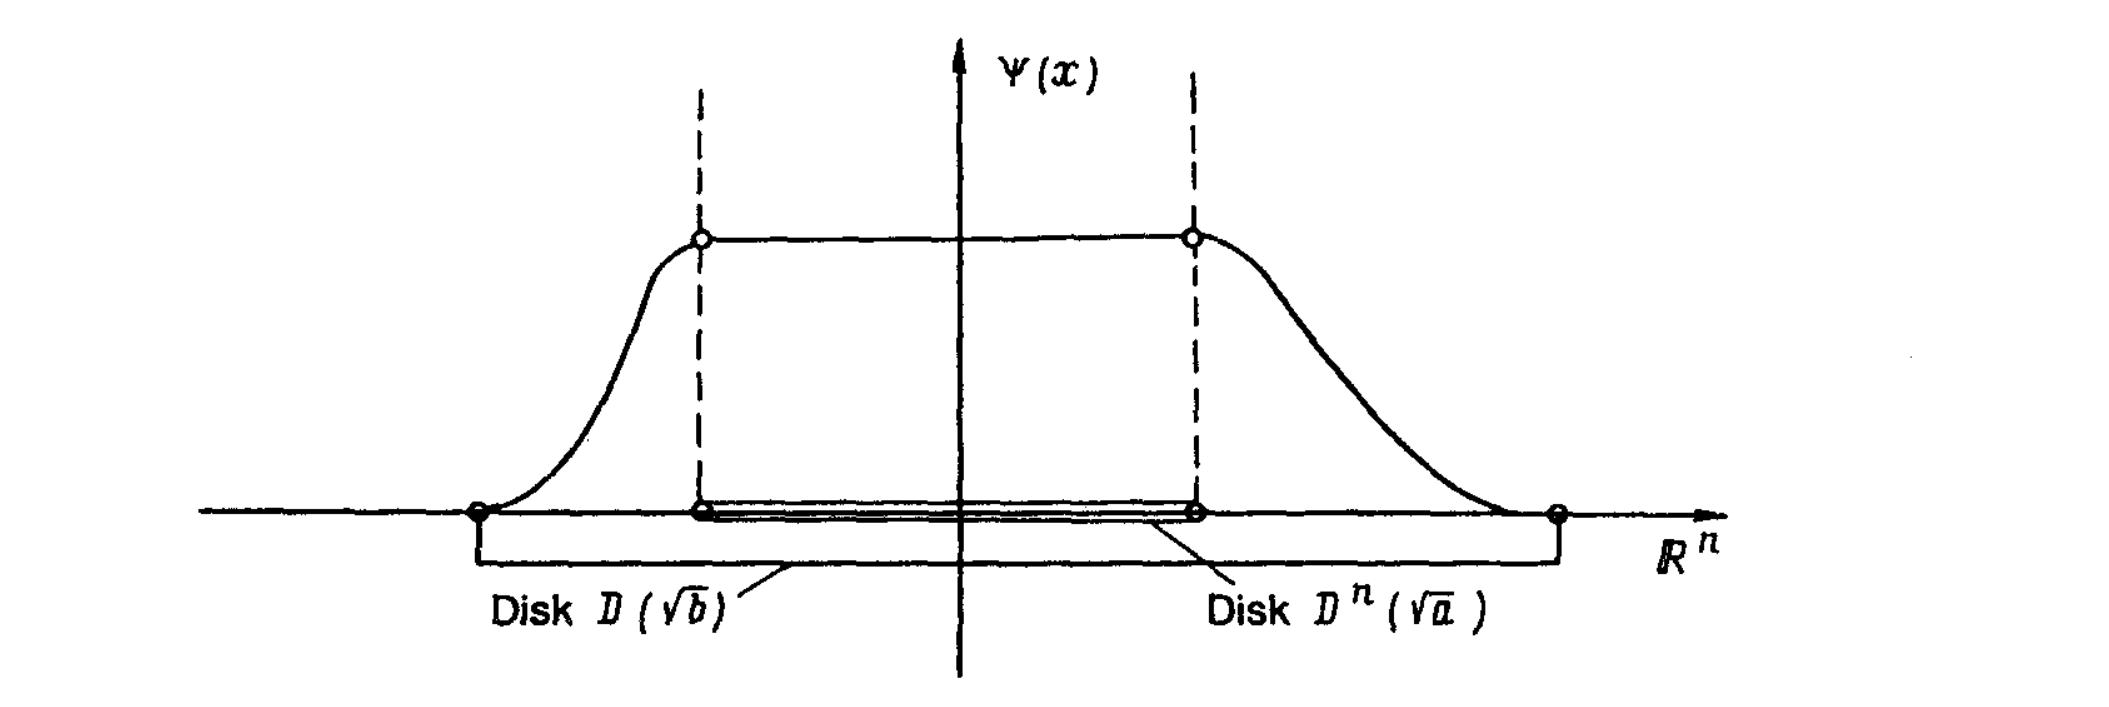
\includegraphics[width=0.82\textwidth]{figures/fig4_1.png}
\end{center}
\figtitle{4.1}{图中：函数 $\psi(x)$ 的图像；横轴为 $\R^n$，两个圆盘分别记作 $D(\sqrt b)$ 与 $D^n(\sqrt a)$。}

% [Tutor Note: 单位分解是光滑流形上把局部构造粘成整体构造的唯一通用工具：后文用积分定义 de Rham 上同调、用联络构造示性类时，都要先取单位分解把局部数据拼起来。]
\begin{example}{}
对紧流形 $M^n$，对由局部坐标邻域组成的一切有限覆盖 $\{V_\alpha\}$，单位分解都存在。若把每个区域 $V_\alpha$ 上的局部坐标 $x_\alpha^j$ 乘以相应单位分解的函数 $\psi_\alpha$（见上文），所得函数记作 $\psi_\alpha x_\alpha^j=y_\alpha^j$，则它们在整个流形 $M^n$ 上有定义且光滑。若覆盖 $\{V_\alpha\}=\{V_1,\ldots,V_N\}$，则函数族 $\{y_\alpha^j\}$（$j=1,\ldots,n$，$\alpha=1,\ldots,N$）定义一个 $C^\infty$-嵌入
\[
\{y_\alpha^j\}:M^n\to\R^{nN},
\]
因为 $\psi_\alpha\equiv1$ 在 $W_\alpha$ 上，而 $W_\alpha$ 中任意两点都可由其局部坐标 $x_\alpha^j$ 区分。对非紧流形，同样的论证给出到 Hilbert 空间的嵌入。利用「一般位置」的思想（见下文）以及把上述嵌入流形投影到 $k$ 维超平面，可以证明：当 $k\ge2n+1$ 时，光滑嵌入 $M^n\to\R^k$ 的集合在光滑（甚至仅连续）映射 $M^n\to\R^k$ 的空间中处处稠密；当 $k\ge2n$ 时，光滑浸入的集合同样处处稠密。当 $n=1$ 时这在直观上很明显——见图 4.2。
\end{example}

两个光滑流形之间的\emph{光滑映射} $f:M^n\to N^k$，是指这样的映射：用 $M^n$ 的坐标卡 $V_\alpha$ 上的局部坐标系 $\{x_\alpha^j\mid j=1,\ldots,n\}$ 与 $N^k$ 的坐标卡 $U_\gamma$ 上的局部坐标系 $\{y_\gamma^s\mid s=1,\ldots,k\}$ 写出它的每个表达式，都是（通常意义下的）光滑函数 $y_\gamma^s(x_\alpha^1,\ldots,x_\alpha^n)$。（这里每个这样的函数的定义域都具有形状
\[
f^{-1}(U_\gamma)\cap V_\alpha.)
\]
在 $M^n$ 的每一点 $x$ 处，光滑映射 $f$ 的\emph{秩}（$\rank f(x)$）定义为矩阵 $(\partial y_\gamma^s/\partial x_\alpha^j)$ 在 $x$ 处的秩。每点处的秩是 $f$ 的不变量（即与所采用的局部坐标无关）。

% [原文 p.144]
\begin{center}
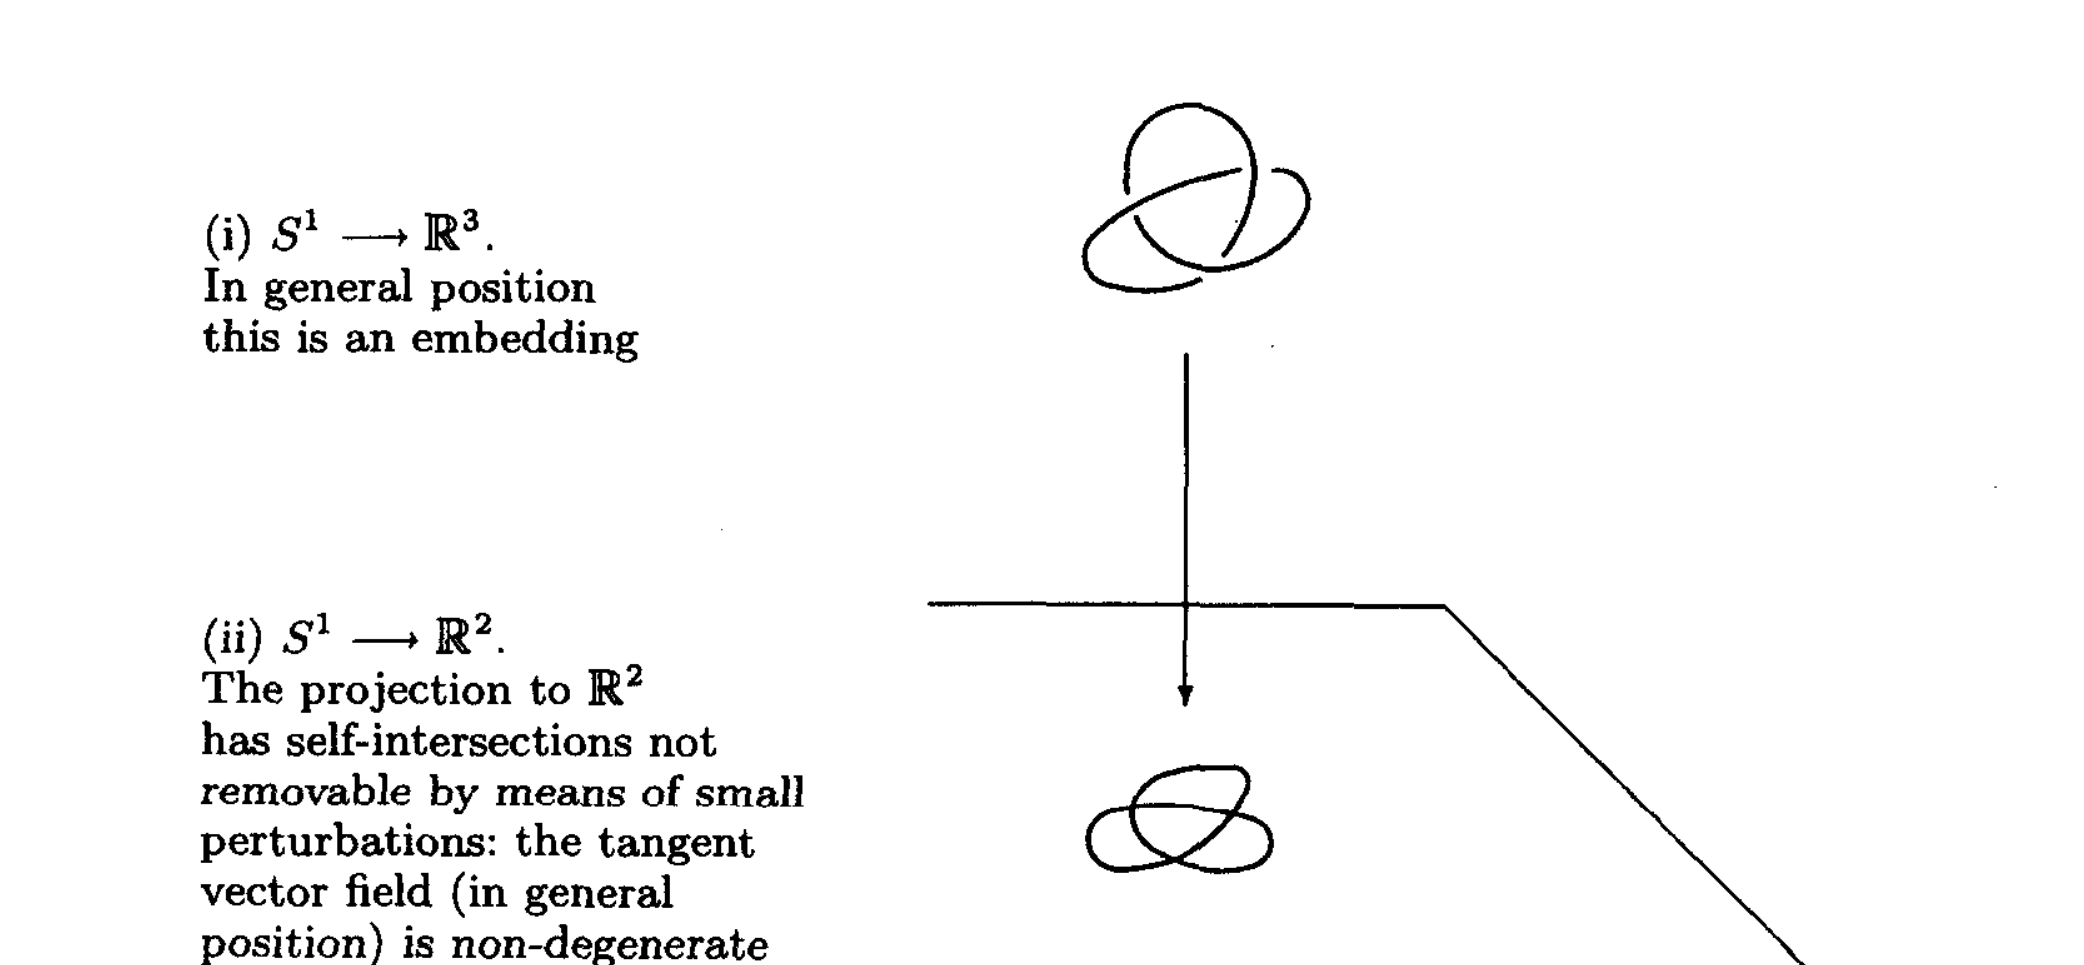
\includegraphics[width=0.72\textwidth]{figures/fig4_2.png}
\end{center}
\figtitle{4.2}{(i) 一般位置下 $S^1\to\R^3$ 是嵌入；(ii) 投影到 $\R^2$ 后自交点不能靠小扰动消去，切向量场（在一般位置下）非退化。}

% [Tutor Note: 上文使用的「一般位置」只有两个要点：$\rank f\ge k$ 的点集是开的稠密集；映射经小扰动后可假定处于横截位置。Whitney 的嵌入定理与 Sard 定理的证明属于微分拓扑，本书只引用结论，不重复证明。]
\emph{浸入} $f:M^n\to N^k$ 是指每点 $x\in M^n$ 处 $f$ 的秩都等于 $n$ 的光滑映射（于是必有 $n\le k$）。\emph{淹没}由条件 $\rank f\equiv k$ 定义（于是 $n\ge k$）。\emph{嵌入}是一一浸入：$x\ne y$ 时 $f(x)\ne f(y)$。两个光滑流形之间的\emph{微分同胚} $f:M_1^n\to M_2^n$ 是逆映射也光滑的光滑同胚。

流形的光滑性类 $C^k$（在 $k\ge1$ 这一基本假定之外）对拓扑学并无太大意义，这依据 Whitney 的一个定理：任何 $C^k$-流形都微分同胚于唯一的 $C^\infty$-流形，事实上微分同胚于唯一的实解析流形。（Morrey 后来（1950 年代后期）还证明了：任何实解析流形都可实解析地嵌入某个 $\R^n$；这是一个困难的结果，需要复流形理论的较新方法。）因此在下文中，我们将经常不加说明地假定所论光滑流形与映射的光滑性类为 $C^\infty$，并且不区分彼此微分同胚的流形。

自 Whitney 起，关于「一般位置」的引理（Brown、Sard 等人也在 1930 年代得到过）在研究光滑流形拓扑的技巧中起了重要作用。其中最简单的一条断言：对光滑性类 $C^k$ 充分高的实值映射 $f:M^n\to\R$，临界点集 $Z$（即使得 $\grad f(x)=0$ 的点 $x\in M^n$）的像 $f(Z)$ 在 $\R$ 中测度为零。（对紧 $M^n$，集合 $f(Z)$ 闭，其补集有正测度。）更一般地，对光滑性类充分高的任意映射 $f:M^n\to N^k$（$k\le n$），其集合 $f(Z)$ 在 $N^k$ 中测度为零，其中 $Z$ 由满足 $\rank f(x)<k$ 的点 $x\in M^n$ 组成。
% [原文 p.145]
又注意对任意 $C^1$-映射 $M^n\to N^k$（$k>n$），像 $f(M^n)$ 在 $N^k$ 中测度为零。在上述各种情形中，位于集合 $f(Z)$ 之外（后一情形 $k>n$ 中位于 $f(M^n)$ 之外）的陪域 $N^k$ 中的点，称为关于 $f$ 处于\emph{一般位置}。把映射调入一般位置的各种重要引理，我们将在需要时叙述。

回忆：$M^n$ 在点 $x_0$ 处的\emph{切向量}，是过 $x_0$ 的参数曲线 $x_\alpha^j(t)$（在包含 $x_0$ 的坐标卡 $V_\alpha$ 上的局部坐标中）在 $x_0$ 处的速度向量 $(dx_\alpha^j/dt)_{x_0}$。$M^n$ 在 $x_0$ 处一切切向量构成的向量空间 $\R^n_{x_0}$ 称为 $M^n$ 在 $x_0$ 处的\emph{切空间}。

设 $(\eta_\alpha^1,\ldots,\eta_\alpha^n)$ 是点 $x\in M^n$ 处任一切向量，用包含 $x$ 的局部坐标邻域上的局部坐标 $x_\alpha^1,\ldots,x_\alpha^n$ 表示。变换到坐标 $x_\beta^1,\ldots,x_\beta^n$（Jacobi 矩阵为 $I_{\alpha\beta}=(\partial x_\beta^k/\partial x_\alpha^j)$）时，切向量的分量按下列规则变换：
\begin{equation}
\eta_\beta^k=\eta_\alpha^j\frac{\partial x_\beta^k}{\partial x_\alpha^j}\qquad\text{（对 }j\text{ 求和）}. \tag{1.1}
\end{equation}
另一方面，梯度、更一般地，由局部坐标写出的微分 1-形式 $\sum\eta_{i\alpha}dx_\alpha^i=\eta_{i\alpha}dx_\alpha^i$，按下列规则变换：
\begin{equation}
\eta_{i\beta}=\eta_{k\alpha}\frac{\partial x_\alpha^k}{\partial x_\beta^i}. \tag{1.2}
\end{equation}

更一般的\emph{$(m,k)$ 型张量}，其分量
\[
T^{i_1\cdots i_m}_{j_1\cdots j_k}
\]
相对于局部坐标 $x_\alpha^1,\ldots,x_\alpha^n$，在坐标变换 $\alpha\to\beta$ 下按适当方式变换（即由 (1.1) 与 (1.2)「外推」而得）。还需要再细致一点。用所关心的点 $x$ 的某邻域内的局部坐标 $x_\alpha^1,\ldots,x_\alpha^n$，$x$ 处切空间有通常的标准基向量 $e_{1\alpha},\ldots,e_{n\alpha}$，对偶空间则有相应的对偶基余向量 $e_\alpha^1,\ldots,e_\alpha^n$，其标量积为 $\langle e_\alpha^i,e_{j\alpha}\rangle=\delta_j^i$（即把每个 $e_\alpha^i$ 作用于 $e_{j\alpha}$）。于是 $\R^n_x$ 中每个向量 $\eta$ 有唯一形状 $\eta_\alpha^je_{j\alpha}\in\R^n_x$，每个余向量 $\eta^*$ 有唯一形状 $\eta_{i\alpha}e_\alpha^i\in\R_x^{n*}$。于是在每一点 $x\in M^n$ 处有 $(m,k)$ 型张量的空间
\[
\underbrace{\R^n_x\otimes\cdots\otimes\R^n_x}_{m}\otimes\underbrace{\R_x^{n*}\otimes\cdots\otimes\R_x^{n*}}_{k},
\]
其标准基（相对于所用局部坐标）由下列表达式组成：
\[
e_{i_1\alpha}\otimes\cdots\otimes e_{i_m\alpha}\otimes e_\alpha^{j_1}\otimes\cdots\otimes e_\alpha^{j_k}.
\]

% [原文 p.146]
点 $x$ 处任一张量（$(m,k)$ 型）都有形状（在局部坐标 $x_\alpha^1,\ldots,x_\alpha^n$ 下）
\[
\bigl(T^{i_1\cdots i_m}_{j_1\cdots j_k}\bigr)=T^{i_1\cdots i_m}_{j_1\cdots j_k}e_{i_1}\otimes\cdots\otimes e_{i_m}\otimes e^{j_1}\otimes\cdots\otimes e^{j_k},
\]
其中采用求和约定（并省略指标 $\alpha$）。基向量 $e_{j\alpha}$ 自然地对应算子 $\partial/\partial x_\alpha^j$，对偶基余向量 $e_\alpha^j$ 对应微分 $dx_\alpha^j$：
\[
e_{j\alpha}\leftrightarrow\partial/\partial x_\alpha^j;\qquad e_\alpha^j\leftrightarrow dx_\alpha^j.
\]

$(m,k)$ 型\emph{张量场}则是给 $M^n$ 的每点 $x$ 指定一个 $(m,k)$ 型张量的光滑函数。

下文将不加说明地使用通常的张量（场）运算（缩并、乘积、指标置换等）以及 Einstein 求和约定（即在单个表达式中同时作为上标与下标出现的指标自动求和）。

只有下指标的反对称张量（更确切地说张量场），即 $(0,k)$ 型张量，特别重要；它们的另一个名称是\emph{微分形式}，由于其用于积分理论，通常如下写出（在局部坐标中）：
\begin{equation}
\Omega_k=\frac1{k!}T_{i_1\cdots i_k}dx^{i_1}\wedge\cdots\wedge dx^{i_k}, \tag{1.3}
\end{equation}
微分形式的外积 $\Omega_k\wedge\Omega_l$ 通过张量积以及使外积反对称的「交替」运算代数地定义：
\[
\Omega_k\wedge\Omega_l=(-1)^{kl}\Omega_l\wedge\Omega_k.
\]
用微分形式的局部记号 (1.3)，外积由结合性、与数可交换以及
\begin{equation}
dx^i\wedge dx^j=-dx^j\wedge dx^i \tag{1.4}
\end{equation}
这些条件唯一确定。

形式上的\emph{微分算子} $d$ 由下列条件定义：

（i）$df=\dfrac{\partial f}{\partial x_\alpha^j}dx_\alpha^j$（局部地），对实值函数 $f$；

（ii）$d(dx^{i_1}\wedge\cdots\wedge dx^{i_k})=0$；

（iii）$d(f\Omega_k)=df\wedge\Omega_k+fd\Omega_k$，$f$ 为任意数量函数。

由此推出
\[
d\circ d=0,\qquad d(\Omega_k\wedge\Omega_l)=d\Omega_k\wedge\Omega_l+(-1)^k\Omega_k\wedge d\Omega_l.
\]

最后我们提到流形 $M^n$ 上\emph{Riemann 度量}或\emph{伪 Riemann 度量}这一重要概念：它是非退化的对称 $(0,2)$ 型张量（场），光滑依赖于 $M^n$ 的点 $x$。在局部坐标 $(x_\alpha^j)$ 中，它有形状 $(g_{ij})$，其中 $g_{ij}=g_{ji}$ 且 $\det(g_{ij})\ne0$。
% [原文 p.147]
这样的张量按自然方式决定切向量对、余向量对（以及一般地任意类型张量对）的对称标量积：
\[
\langle\eta_1,\eta_2\rangle=\eta_1^i\eta_2^jg_{ij},
\]
\[
\langle\eta_1^*,\eta_2^*\rangle=\eta_{1i}^*\eta_{2j}^*g^{ij},\qquad g^{ij}g_{jk}=\delta_k^i.
\]
作为研究流形拓扑的工具，通常使用 Riemann 度量，即满足 $\det(g_{ij})>0$ 的度量。但伪 Riemann 度量也屡见不鲜；它们不仅在相对论中重要，在研究半单 Lie 群的几何时也很重要。

\emph{Lie 群}是装备了光滑二元运算
\[
\psi:M^n\times M^n\to M^n;\qquad \psi(x,y)=x\cdot y,\quad x,y\in M^n
\]
的光滑流形 $M^n$，在此运算下 $M^n$ 成群：$(x\cdot y)\cdot z=x\cdot(y\cdot z)$；有单位元 $1$；每个元素 $x$ 有逆元 $x^{-1}$（$xx^{-1}=x^{-1}x=1$），且逆元应光滑依赖于 $x$。

设 $x^1,\ldots,x^n$ 是 Lie 群 $M^n$ 在 $x_0=1$ 邻域内的局部坐标。用这样的坐标，群运算 $z=\psi(x,y)$ 具有形状
\[
z^j=\psi^j(x^1,\ldots,x^n,y^1,\ldots,y^n),
\]
于是由 Taylor 定理
\begin{equation}
\begin{gathered}
z^j=x^j+y^j+b_{ks}^jx^ky^s+o(|x|\cdot|y|),\\
(x^{-1})^j=-x^j+o(|x|).
\end{gathered}\tag{1.5}
\end{equation}

Lie 群 $M^n$ 的\emph{Lie 代数}是 $M^n$ 在 $x_0=1$ 处的切空间，装备了如下定义的换位运算（用 $1$ 邻域内的局部坐标表示）：
\begin{equation}
[\xi,\eta]^k=(b_{js}^k-b_{sj}^k)\xi^j\eta^s, \tag{1.6}
\end{equation}
其中 $\xi=(\xi^1,\ldots,\xi^n)$，$\eta=(\eta^1,\ldots,\eta^n)$。立刻看出该运算是双线性的、反对称的（$[\xi,\eta]=-[\eta,\xi]$），并满足 Jacobi 恒等式：
\begin{equation}
[[\xi,\eta],\zeta]+[[\eta,\zeta],\xi]+[[\zeta,\xi],\eta]=0. \tag{1.7}
\end{equation}
最重要的 Lie 群是各种域上的矩阵群，特别是 $\R$、$\C$ 以及四元数斜域 $\HH$ 上的矩阵群。群 $O_{p,q}$ 由向量空间 $\R^n$（$n=p+q$）中保符号差为 $p,q$ 的对称标量积的线性变换组成。

% [原文 p.148]
\emph{正交群} $O_n$（$=O_{n,0}$）当然特别重要。类似地，群 $U_{p,q}$ 由 $\C^n$（$n=p+q$）中保符号差为 $(p,q)$ 的 Hermite 标量积的线性变换组成，而 $U_n=U_{n,0}$ 是\emph{酉群}。相应的子群 $SO_{p,q}$、$SO_n$、$SU_{p,q}$、$SU_n$ 以及 $SL_n(\R)\subset GL_n(\R)$、$SL_n(\C)\subset GL_n(\C)$（其中 $SG$ 表示矩阵群 $G$ 中行列式为 $1$ 的子群）也很重要。最后，$Sp_n$ 表示 $n\times n$ 四元数正交矩阵组成的子群。Lie 群 $O_n$、$U_n$、$SO_n$、$SU_n$、$Sp_n$ 都紧，并且由 Cartan--Killing 定理，不局部同构于上列矩阵群中某个群的紧、单连通、单 Lie 群只有有限多个（即 $6$ 个）。事实上每个紧 Lie 群 $G$ 都有形状
\[
(T^n\times G_1\times G_2\times\cdots\times G_k)/D,
\]
其中 $T^n$ 是 $n$-环面，$G_i$ 是紧、单连通、单 Lie 群（从而出现在 Cartan--Killing 表中），$D$ 是中心内的有限子群。

% [Tutor Note: 这里列出的 Lie 群与 (1.8)(1.9) 的齐性空间，是下一章把「丛的分类」化为「同伦类」的全部原料：$O_n$、$U_n$ 给出向量丛的结构群，$SO_n$、$SU_n$ 对应定向情形。]
\emph{光滑纤维丛}像一般情形那样定义（见第 3 章 §6），只是现在要求空间 $E$、$B$、$F$ 都是光滑流形，投影 $p$ 是光滑映射，衔接函数也光滑，且结构群 $G\subset\Diff F$，即纤维 $F$ 的微分同胚群的子群。（在最重要的场合，$G$ 是 Lie 群。）

\emph{（光滑）向量丛}是纤维 $F$ 为向量空间、结构群 $G$ 作为线性变换群作用于其上的光滑纤维丛。两种最重要的类型是\emph{实向量丛}，其中 $F\cong\R^n$、$G\subset GL_n(\R)$，以及\emph{复向量丛}，其中 $F\cong\C^n$、$G\subset GL_n(\C)$。

一个重要的例子是光滑流形 $M^n$ 的\emph{切丛} $\tau=\tau(M^n)$，其中 $F\cong\R^n$、$G=GL_n(\R)$、底为 $B=M^n$；全空间记作 $T(M^n)$。注意切丛的截面正是 $M^n$ 上的（切）向量场。若 $M$ 上给定 Riemann 度量，则结构群约化为 $O_n$。

由 $M^n$ 上的切丛可以构造许多重要的、$M^n$ 上的相伴向量丛，其纤维上带有群 $GL_n(\R)$ 的作用。例如取每点 $x\in M^n$ 处的对偶空间 $\R_x^{n*}$ 为纤维（即 $(0,1)$ 型张量的空间），得到\emph{余切向量丛} $\tau^*$，全空间记作 $T^*(M^n)$。更一般地，群 $GL_n(\R)$ 在 $(m,k)$ 型张量空间上的作用，给出 $M^n$ 上以该张量空间为纤维的相伴向量丛；此丛记作
\[
\underbrace{\tau\otimes\cdots\otimes\tau}_{m\ \text{次}}\otimes\underbrace{\tau^*\otimes\cdots\otimes\tau^*}_{k\ \text{次}}.
\]

% [原文 p.149]
类似地，可以作余切空间 $\tau^*$ 的外幂 $\Lambda^k(\tau^*)$。于是 $M^n$ 上的微分形式就是这种向量丛的截面。$M^n$ 上的 Riemann 度量类似地可看作切丛对称平方 $S^2\tau$（即 $\tau\otimes\tau$ 的对称部分）的截面。

与切空间相伴的向量丛还有一个例子：每点之上的纤维由线性无关切向量的有序 $k$-组（$k$-标架）组成。

在给定 Riemann 度量时，宜使用群 $O_n$（而非 $GL_n(\R)$）通过纤维上的线性变换给出的表示。正交群与酉群的重要齐性空间是 \emph{Stiefel 流形}与 \emph{Grassmann 流形}。实（或复）Stiefel 流形 $V^{\R}_{n,k}$（或 $V^{\C}_{n,k}$）的点是 $\R^n$（或带 Hermite 度量的 $\C^n$）中的正交 $k$-标架 $(v_1,\ldots,v_k)$。容易看出
\begin{equation}
\begin{gathered}
V^{\R}_{n,k}\cong SO_n/SO_{n-k}\cong O_n/O_{n-k},\\
V^{\C}_{n,k}\cong SU_n/SU_{n-k}\cong U_n/U_{n-k}.
\end{gathered}\tag{1.8}
\end{equation}
实（或复）Grassmann 流形 $G^{\R}_{n,k}$（或 $G^{\C}_{n,k}$）的点是 $\R^n$（或 $\C^n$）的 $k$ 维子空间。由于 $O_n$ 在 $\R^n$ 上的通常作用诱导出该群在全部 $k$ 维子空间集合上的可迁作用（$U_n$ 在 $\C^n$ 上类似），不难推出
\begin{equation}
\begin{gathered}
G^{\R}_{n,k}\cong SO_n/(SO_{n-k}\times SO_k)\cong O_n/(O_{n-k}\times O_k),\\
G^{\C}_{n,k}\cong SU_n/(SU_{n-k}\times SU_k)\cong U_n/(U_{n-k}\times U_k).
\end{gathered}\tag{1.9}
\end{equation}

\emph{可定向 Grassmann 流形} $\widehat{G}^{\R}_{n,k}$ 的点是 $\R^n$ 的定向 $k$ 维子空间。它是相应 Grassmann 流形 $G^{\R}_{n,k}$ 的二重覆叠（纤维为 $\Z/2$）：
\[
\widehat{G}^{\R}_{n,k}\to G^{\R}_{n,k}.
\]
有自然的嵌入
\[
G^{\R}_{n,k}\to G^{\R}_{n+1,k},\qquad \widehat{G}^{\R}_{n,k}\to\widehat{G}^{\R}_{n+1,k},\qquad G^{\C}_{n,k}\to G^{\C}_{n+1,k},
\]
它们由标准嵌入 $\R^n\to\R^{n+1}$、$\C^n\to\C^{n+1}$ 诱导。把相应空间与嵌入序列的正向极限记作 $G^{\R}_k$、$\widehat{G}^{\R}_k$、$G^{\C}_k$：
\[
G^{\R}_k=\lim_{n\to\infty}G^{\R}_{n,k},\qquad \widehat{G}^{\R}_k=\lim_{n\to\infty}\widehat{G}^{\R}_{n,k},\qquad G^{\C}_k=\lim_{n\to\infty}G^{\C}_{n,k}.
\]
容易直接看出 $\widehat{G}^{\R}_1$ 可缩、$G^{\R}_1=\RP^\infty$、$G^{\C}_1=\CP^\infty$。

% [原文 p.150]
由下文同构 (1.13)，可得
\begin{equation}
\begin{gathered}
\pi_j(V^{\R}_{n,k})=0\quad \text{当}\ j<n-k,\\
\pi_j(V^{\C}_{n,k})=0\quad \text{当}\ j<2(n-k).
\end{gathered}\tag{1.10}
\end{equation}
主丛
\begin{equation}
\begin{gathered}
E^{\R}_n=V^{\R}_{n,k}\to G^{\R}_{n,k},\qquad F=O_k=G,\\
\widehat{E}^{\R}_n=V^{\R}_{n,k}\to\widehat{G}^{\R}_{n,k},\qquad F=SO_k=G,\\
E^{\C}_n=V^{\C}_{n,k}\to G^{\C}_{n,k},\qquad F=U_k=G,
\end{gathered}\tag{1.11}
\end{equation}
（其中投影是显然的那些）连同空间
\[
E^{\R}_\infty=\lim_{n\to\infty}E^{\R}_n,\qquad \widehat{E}^{\R}_\infty=\lim_{n\to\infty}\widehat{E}^{\R}_n,\qquad E^{\C}_\infty=\lim_{n\to\infty}E^{\C}_n
\]
可缩这一观察，导致如下结论：

\emph{主丛 (1.11) 当 $n\to\infty$ 时的极限给出 Lie 群 $G=O_k,SO_k,U_k$ 的万有 $G$-丛。于是这些群的分类空间为}
\begin{equation}
BO_k=G^{\R}_k,\qquad BSO_k=\widehat{G}^{\R}_k,\qquad BU_k=G^{\C}_k. \tag{1.12}
\end{equation}

回忆：任一映射 $M^n\to BG$ 通过拉回丛决定 $M^n$ 上一个（主）$G$-丛，且在同伦意义下唯一（这给出 $M^n$ 上（主）$G$-丛的等价类与映射 $M^n\to BG$ 的同伦类集合 $[M^n,BG]$ 之间的一一「分类」对应）。对 $M^n$ 的切丛，相应的映射 $M^n\to BO_k$（或 $M^n\to BSO_k$）自然地出现，作为曲面的球面 Gauss 映射的推广。先把 $M^n$ 嵌入 $\R^N$（$N$ 充分大，由 Whitney 定理可以做到），然后把 $M^n$ 的每点 $x$ 与 $M^n$ 在 $x$ 处的切平面（若 $M^n$ 可定向则带所指的定向）平行移动到 $\R^N$ 的原点相联系。这定义出适当的分类映射
\[
f:M^n\to G^{\R}_{N,n}\quad \Bigl(\text{或}\ f:M^n\to\widehat{G}^{\R}_{N,n},\ \text{若}\ M^n\ \text{可定向}\Bigr),
\]
它自然地被从 $M^n$ 的切丛到万有丛的诱导映射所覆叠。

把这一构造推广到以流形 $B$ 为底的任意光滑向量丛并无困难。注意这种丛的全空间 $E$ 可缩到 $B$（与零截面等同）。把 $E$ 嵌入 $\R^N$（$N$ 适当大），并考察 $B\subset E$ 的每一点处的平面（该平面在 $\R^N$ 中于 $x$ 处与过 $x$ 的纤维 $F_x\subset\R^N$ 相切）。
% [原文 p.151]
把这些平面平行移动到 $\R^N$ 的原点，便得到所需映射 $B\to G^{\R}_{N,n}$（或 $B\to\widehat{G}^{\R}_{N,n}$，若 $B$ 可定向）。由于任意有限 CW 复形 $K$ 都有同伦等价的光滑流形 $U$（把 $K$ 嵌入某个 $\R^N$，取 $K$ 的以 $K$ 为形变收缩核的小邻域即可），上述由向量丛决定光滑 Gauss 映射的构造，本质上不比有限 CW 复形上万有 $G$-丛的构造更特殊。

对结构群 $G\subset\Diff F$ 的一般光滑纤维丛，万有 $G$-丛可如下构造。记 $E_N(F)$ 为嵌入 $F\to\R^N$ 的空间。群 $\Diff F$ 显然作用于 $E_N(F)$ 上，且正向极限 $E_\infty(F)=\lim_{N\to\infty}E_N(F)$ 可缩。$G$ 在 $E_\infty(F)$ 上作用的轨道空间便给出万有 $G$-丛的底 $BG$。文献中通常采用另一种构造（由 Milnor 于 1950 年代后期给出），它基于不同的想法，可对很广的一类群 $G$ 构造 $BG$。

回到向量丛，注意下列主丛的同伦正合列：
\[
SO_{n-1}\to SO_n\to SO_n/SO_{n-1}\cong S^{n-1},
\]
\[
U_{n-1}\to U_n\to U_n/U_{n-1}\cong S^{2n-1}
\]
（其中 $SO_{n-1}\to SO_n$、$U_{n-1}\to U_n$ 是嵌入），连同当 $j\le k-2$ 时 $\pi_j(S^{k-1})$ 平凡这一事实，给出同构：
\begin{equation}
\begin{gathered}
\pi_k(SO_n)\cong\pi_k(SO_{n-1}),\qquad k<n-1,\\
\pi_k(U_n)\cong\pi_k(U_{n-1}),\qquad k<2(n-1).
\end{gathered}\tag{1.13}
\end{equation}
于是自然嵌入 $SO_{n-k}\to SO_n$、$U_{n-k}\to U_n$（以及 $SU_{n-k}\to SU_n$）在维数分别小于 $n-k-1$、$2(n-k)$ 的同伦群之间诱导同构。由此即得上文 (1.10)。（对 $Sp_n$ 类似地有 $\pi_k(Sp_n)\cong\pi_k(Sp_{n-1})$，$k<4n-2$。）同伦群 $\pi_k(O_n)\cong\pi_k(SO_n)$（$k<n-1$）、$\pi_k(U_n)$（$k<2n-2$）、$\pi_k(Sp_n)$（$k<4n-2$）称为\emph{稳定的}，因为在这些范围内它们与 $n$ 无关。它们最早由 Bott（1950 年代后期）用整体变分法算出（见下文 §2）。

结构群为 Lie 群 $G$ 的光滑 $G$-丛的微分几何，关键依赖于「联络」这一概念。流形 $B$（$\dim B=n$）上主 $G$-丛的\emph{微分几何 $G$-联络}，是这样一个光滑 $G$-不变场：对全空间 $E$ 的每一点，指定 $E$ 的切空间的一个 $n$ 维子空间，它与过该点的纤维横截。（回忆 $G$ 自由作用于 $E$，作用的轨道即纤维 $F\cong G$。）附着在 $E$ 各点上的这些 $n$ 维子空间称为\emph{水平的}。

% [原文 p.152]
Lie 群 $G$ 上有标准的右不变 1-形式 $\omega_0$，其值（在 $G$ 的切向量处）取在 $G$ 的 Lie 代数 $\cG$ 中，其中 $\cG$ 等同于 $G$ 上右不变向量场的代数；具体说，$\omega_0$ 在 $x\in G$ 处的每个切向量 $\eta$ 上取值，等于满足 $\xi(x)=\eta$ 的唯一右不变向量场 $\xi$。这个 1-形式满足
\begin{equation}
-\frac12[\omega_0,\omega_0]=d\omega_0,\qquad g^*\omega_0=(\mathrm{Ad}\,g)\omega_0, \tag{1.14}
\end{equation}
其中 $g$ 通过左乘 $h\mapsto gh$ 作用，$[\,,\,]$ 表示 $G$ 上取值于 $\cG$ 的形式的外积运算。（回忆：取值于任意环的形式与上链都可以相乘，尽管一般说来乘法不是反交换的。又注意：对矩阵 Lie 群 $G$，矩阵 Lie 代数 $\cG$ 的线性变换 $\mathrm{Ad}\,g$ 由用 $g$ 共轭矩阵 $u\in\cG$ 实现：$\mathrm{Ad}\,g(u)=gug^{-1}$。）主丛 $(E,B,G,\cG,p)$ 上的联络，于是由 $E$ 上任意一个取值于 Lie 代数 $\cG$ 的 1-形式 $\omega$ 确定，只要它满足
\begin{equation}
g^*\omega=(\mathrm{Ad}\,g)\omega,\qquad \omega|F=\omega_0, \tag{1.15}
\end{equation}
其中 $F$（$\cong G$）是任一点之上的纤维；$E$ 的每点 $y$ 处的水平 $n$ 维切子空间，由 $y$ 处的方程 $\omega=0$ 定义。可以证明：反之，$G$-丛上任一联络都确定这样的 1-形式 $\omega$。

$E$ 上的\emph{曲率形式} $\Omega$ 是由下式定义的 2-形式：
\begin{equation}
\Omega=d\omega+\frac12[\omega,\omega]. \tag{1.16}
\end{equation}
由此可知对所有 $g\in G$ 有 $g^*\Omega=(\mathrm{Ad}\,g)\Omega$。此外，形式 $\Omega$ 如他们所说「纯水平的」：它在任意一对切向量（其中至少一个竖直，即与该点处纤维相切）上为零。于是 $\Omega$ 本质上只在「水平」切向量对上取非零值。

设 $x^1,\ldots,x^n$ 是任一（标准）坐标卡 $U\subset B$ 上的坐标，该坐标卡满足 $p^{-1}(U)\cong U\times G$（比如经由 $\phi_U$）。这些坐标于是给出 $U\times\{1\}$ 上的坐标；用这样的局部坐标，联络的形式 $\omega$ 限制到 $U\times\{1\}$ 上为
\[
\omega_{\phi_U}=\omega|_{U\times\{1\}}=A_adx^a,
\]
（其中 $A_a$ 是点 $(x^a)$ 的 $\cG$-值函数），而曲率形式 $\Omega$ 局部形如
\[
\Omega_{\phi_U}=\Omega|_{U\times\{1\}}=F_{ab}dx^a\wedge dx^b,
\]
其中 $F_{ab}$ 是 $(x^a)$ 的 $\cG$-值函数。由 (1.16) 推出
\begin{equation}
F_{ab}=\partial_aA_b-\partial_bA_a+[A_a,A_b],\qquad \partial_a=\partial/\partial x^a. \tag{1.17}
\end{equation}

% [Tutor Note: 联络有两种等价说法：几何说法是「水平 $n$ 维子空间场」，代数说法是「Lie 代数值 $1$-形式 $\omega$」。(1.15) 的第二个条件是 $\omega$ 在纤维上的限制等于 Maurer--Cartan 形式 $\omega_0$，(1.14) 则是 $\omega_0$ 的结构方程。]
% [Tutor Note: (1.17) 就是 Cartan 结构方程在局部坐标下的写法：$\Omega=d\omega+\frac12[\omega,\omega]$ 展开后，末项是 Lie 代数括积而非张量的对称化，注意不要与 (1.2) 的指标变换混淆。]

% CHUNK ch04a DONE
